\documentclass[14pt]{extreport}
\usepackage{cmap}
\usepackage[utf8]{inputenc}
\usepackage[english,ukrainian]{babel}
\usepackage{graphicx}
\usepackage{geometry}
\usepackage{listings}
\usepackage{amsmath}
\usepackage{float}
\geometry{
	a4paper,
	left=20mm,
	right=20mm,
	top=20mm,
	bottom=20mm
}
\lstset{
	language=bash,
	tabsize=4,
	breaklines,
	keepspaces,
	showstringspaces=false,
}
\graphicspath{ {./pictures} }
\setlength{\parindent}{4em}

\newcommand\subject{Бази даних}
\newcommand\lecturer{асистент кафедри ПЗ\\Білоіваненко М.В.}
\newcommand\teacher{асистент кафедри ПЗ\\Майхер В.Ю.}
\newcommand\mygroup{ПЗ-32}
\newcommand\lab{1}
\newcommand\theme{Встановлення та налаштування PostgreSQL та PgAdmin}
\newcommand\purpose{Встановити та налаштувати PostgreSQL та PgAdmin}

\begin{document}
\begin{normalsize}
	\begin{titlepage}
		\thispagestyle{empty}
		\begin{center}
			\textbf{МІНІСТЕРСТВО ОСВІТИ І НАУКИ УКРАЇНИ\\
				НАЦІОНАЛЬНИЙ УНІВЕРСИТЕТ "ЛЬВІВСЬКА ПОЛІТЕХНІКА"}
		\end{center}
		\begin{flushright}
			Інститут \textbf{КНІТ}\\
			Кафедра \textbf{ПЗ}
		\end{flushright}
		\vspace{200pt}
		\begin{center}
			\textbf{ЗВІТ}\\
			\vspace{10pt}
			До лабораторної роботи № \lab\\
			\textbf{На тему}: “\textit{\theme}”\\
			\textbf{З дисципліни}: “\subject”
		\end{center}
		\vspace{40pt}
		\begin{flushright}
			
			\textbf{Лектор}:\\
			\lecturer\\
			\vspace{10pt}
			\textbf{Виконав}:\\
			
			студент групи \mygroup\\
			Коваленко Д.М.\\
			\vspace{10pt}
			\textbf{Прийняв}:\\
			
			\teacher\\
			
			\vspace{28pt}
			«\rule{1cm}{0.15mm}» \rule{1.5cm}{0.15mm} 2023 р.\\
			$\sum$ = \rule{1cm}{0.15mm}……………\\
			
		\end{flushright}
		\vspace{\fill}
		\begin{center}
			\textbf{Львів — 2023}
		\end{center}
	\end{titlepage}
		
	\begin{description}
		\item[Тема.] \theme.
		\item[Мета.] \purpose.
	\end{description}

	\section*{Лабораторне завдання}
	\begin{enumerate}
		\item Встановити та налаштувати PostgreSQL та PgAdmin.
	\end{enumerate}
	
	\section*{Хід роботи}
	Я виконав наступні 3 команди для встановлення бази даних PostgreSQL та PgAdmin.
	\subsection*{1. Створення групи контейнерів \textit{lpnu-db}}
	Створю групу контейнерів з назвою \textit{lpnu-db} та переадресацією порту 80 на 8080 для доступу поза контейнерами.
	\begin{lstlisting}
		podman pod create --name lpnu-db -p 8080:80
	\end{lstlisting}
	
	\subsection*{2. Створення контейнера бази даних}
	Створю контейнер з базою даних що буде належати до групи \textit{lpnu-db} та мати значення паролю, ім'я користувача, назви бази даних за замовчуванням.
	\begin{lstlisting}
		podman run --pod=lpnu-db -e POSTGRES_PASSWORD=password -e POSTGRES_USER=user --name db -d postgres
	\end{lstlisting}
	
	\subsection*{3. Створення контейнера PgAdmin}
	Створю контейнер з \textit{PgAdmin} що буде належати до групи \textit{lpnu-db} та мати значення емайлу та паролю користувача за замовчуванням.
	\begin{lstlisting}
		podman run --pod=lpnu-db --env='PGADMIN_DEFAULT_EMAIL=user@domain.com' --env='PGADMIN_DEFAULT_PASSWORD=password' dpage/pgadmin4
	\end{lstlisting}
	
	\begin{figure}[H]
		\centering
		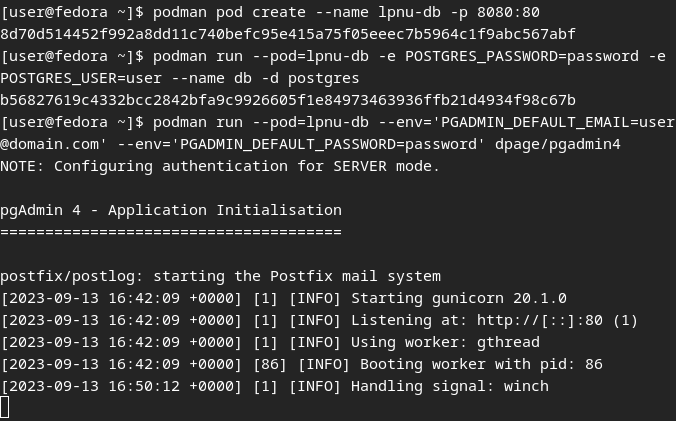
\includegraphics[scale=0.6]{1}
		\caption{Виконання вищезгаданих команд}
	\end{figure}
	
	Тепер \textit{PgAdmin} з підключеною базою даних \textit{PostgreSQL} доступна для використання відкривши посилання \textit{127.0.0.1:8080} у будь-якому браузері.

	
	\begin{figure}[H]
		\centering
		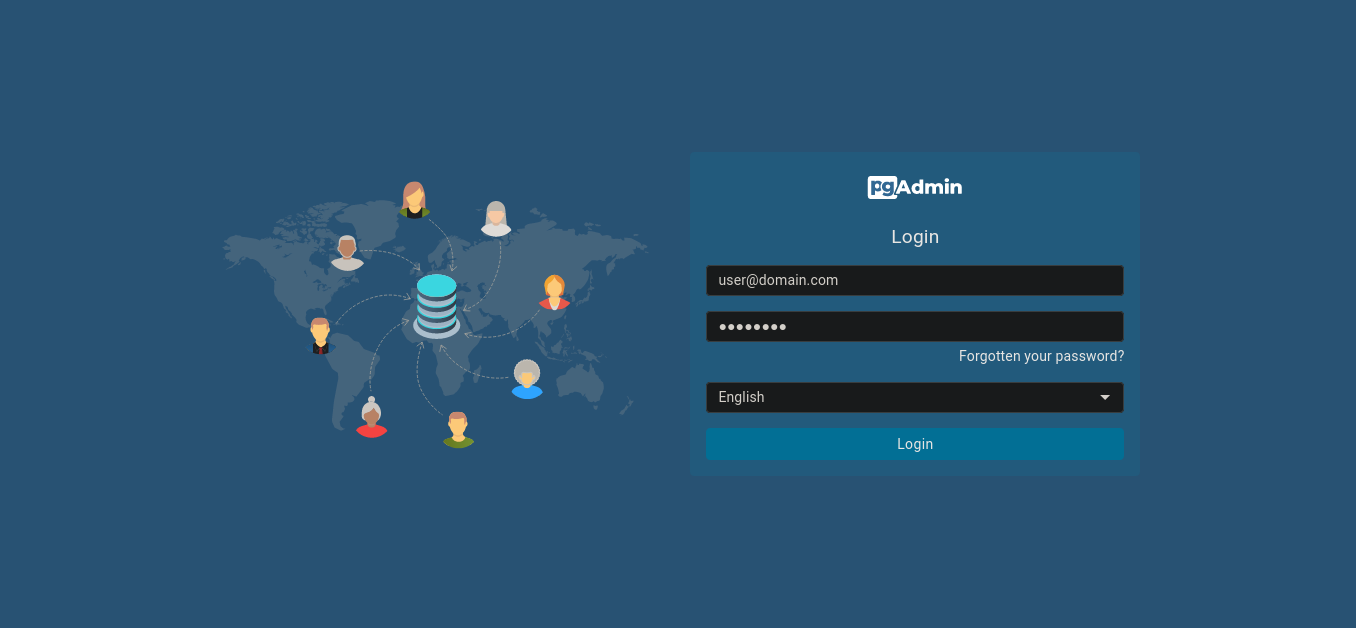
\includegraphics[scale=0.35]{2}
		\caption{Сторінка для авторизації у PgAdmin}
	\end{figure}


	\begin{figure}[H]
		\centering
		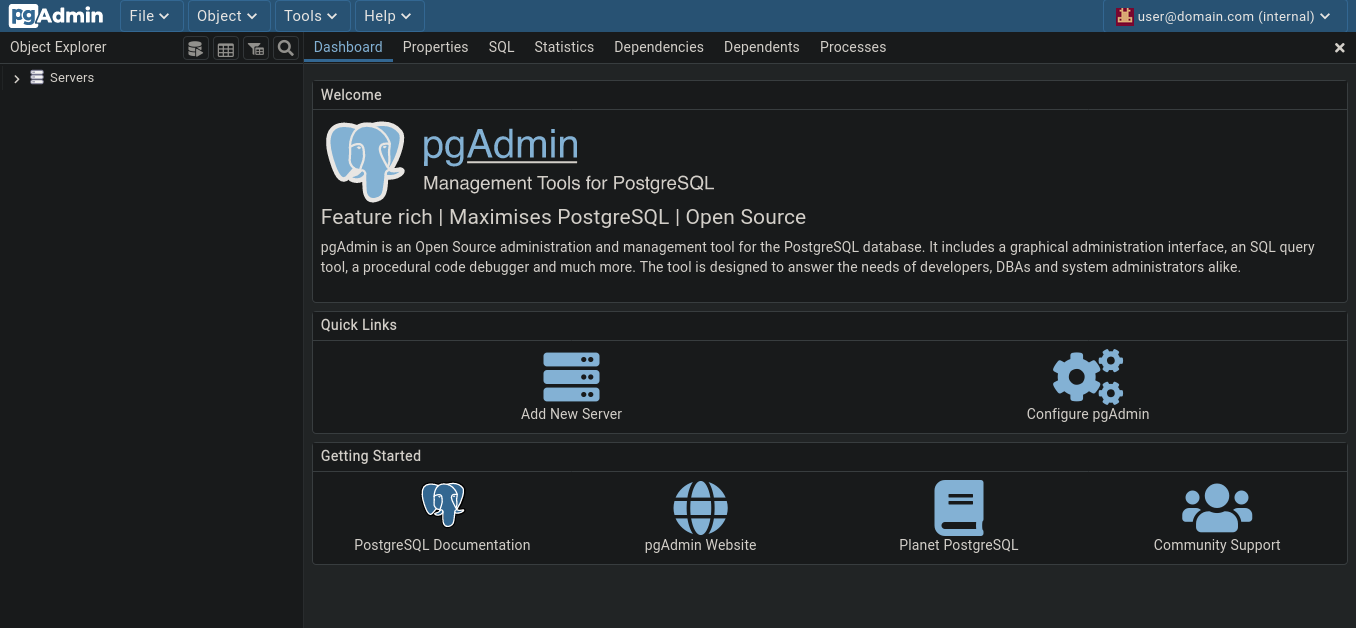
\includegraphics[scale=0.35]{3}
		\caption{Вигляд PgAdmin після входу}
	\end{figure}

	\section*{Висновок}
	Під час виконання лабораторної роботи я встановив та налаштував PostgreSQL та PgAdmin. Для виконання лабораторної роботи я обрав шлях для встановлення та налаштування необхідних програмних компонентів за допомогою контейнеризованого оточення. Я здобув необхідні навички для роботи з PostgreSQL та pgAdmin.
	 
\end{normalsize}
\end{document}
